\section{Design Requirements \& Hardware Implementation} \label{sec:hardware}\label{sec:design_requirements}

\subsection{Purpose}
CALibration Insertion System (CALIS) deploys radioactive gamma and neutron sources inside the LSV to study and calibrate TPC and LSV detector response and neutron detection efficiency. This complements and extends internal calibration sources' and laser calibration's physics reach. 
%The goal with the CALibration source Insertion System (CALIS) is to study and calibrate the detector response of the \tpc\ and the \lsv\ as well as the detection efficiency of internal neutrons interacting in the \tpc\ and \lsv\ using radioactive gamma and neutron sources. 

\lsv's center is about 6 m below gate valve inside CRH
%=6145=70+120+400+3455+20+251+1372+457 from http://darkside-docdb.fnal.gov:8080/cgi-bin/RetrieveFile?docid=858&filename=NoFlyZone-DS50_vers02.pdf&version=14
 and 15 cm diameter wide organ pipes are 80 cm off \tpc's vertical Z-axis as shown in Fig.~\ref{fig:CALIS_photos}. For \tpc\ calibration the radioactive source has to be positioned in immediate contact with cryostat, in order to minimize rate losses through absorption in particular for low energy sources such as $^{57}$Co (122 keV). 

\subsection{Deployment \& Articulation Mechanism}\label{sec:DeploymentArticulation}
%focus on the mechanism --- protection provided by the housing is discussed below:
This requirement precludes a single cable solution deployed from within a glove box used in several scintillator experiments \cite{Banks:2014hra, Huang:2013uxa}. %\cite{KamLAND-MiniCal, DayaBay_zaxis}. 
As shown in Figs. \ref{fig:CALIS_photos} and \ref{fig:CALISMechanism} this apparatus consists instead of an enclosure, which has been installed in CRH and the deployment device is attached to enclosure through two stainless steel cables wound up on cable spools and allow lowering of device into \lsv, next to cryostat.
\begin{figure}[htbp]
 \centering
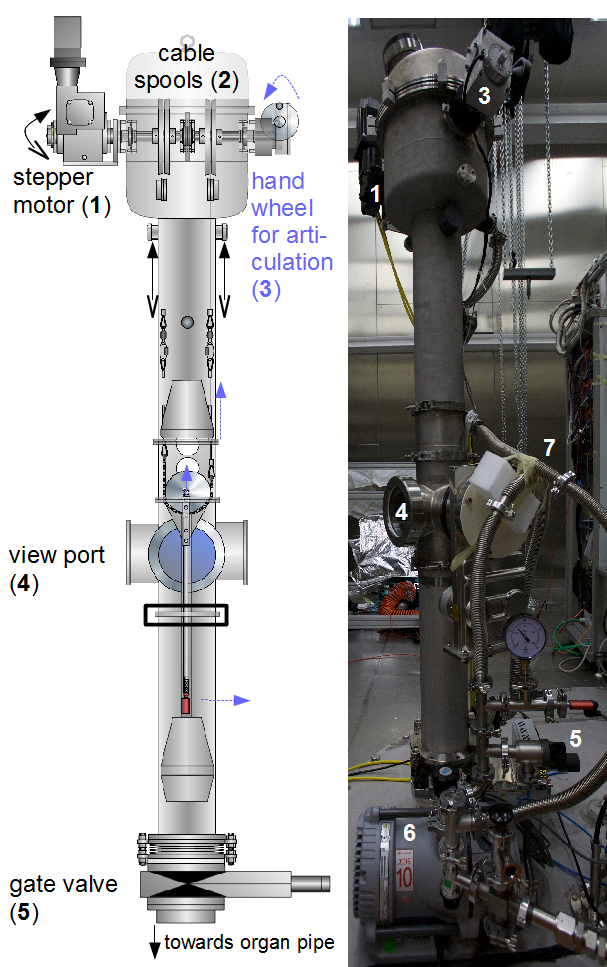
\includegraphics[width=0.8\textwidth]{Figures/CALIS_overview.png}
 %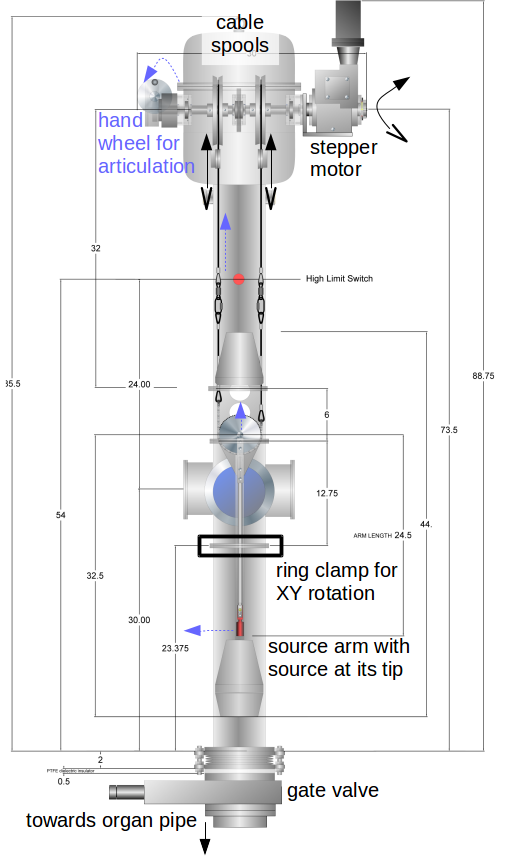
\includegraphics[width=0.68\textwidth]{Figures/CALISDimensions.png}
 %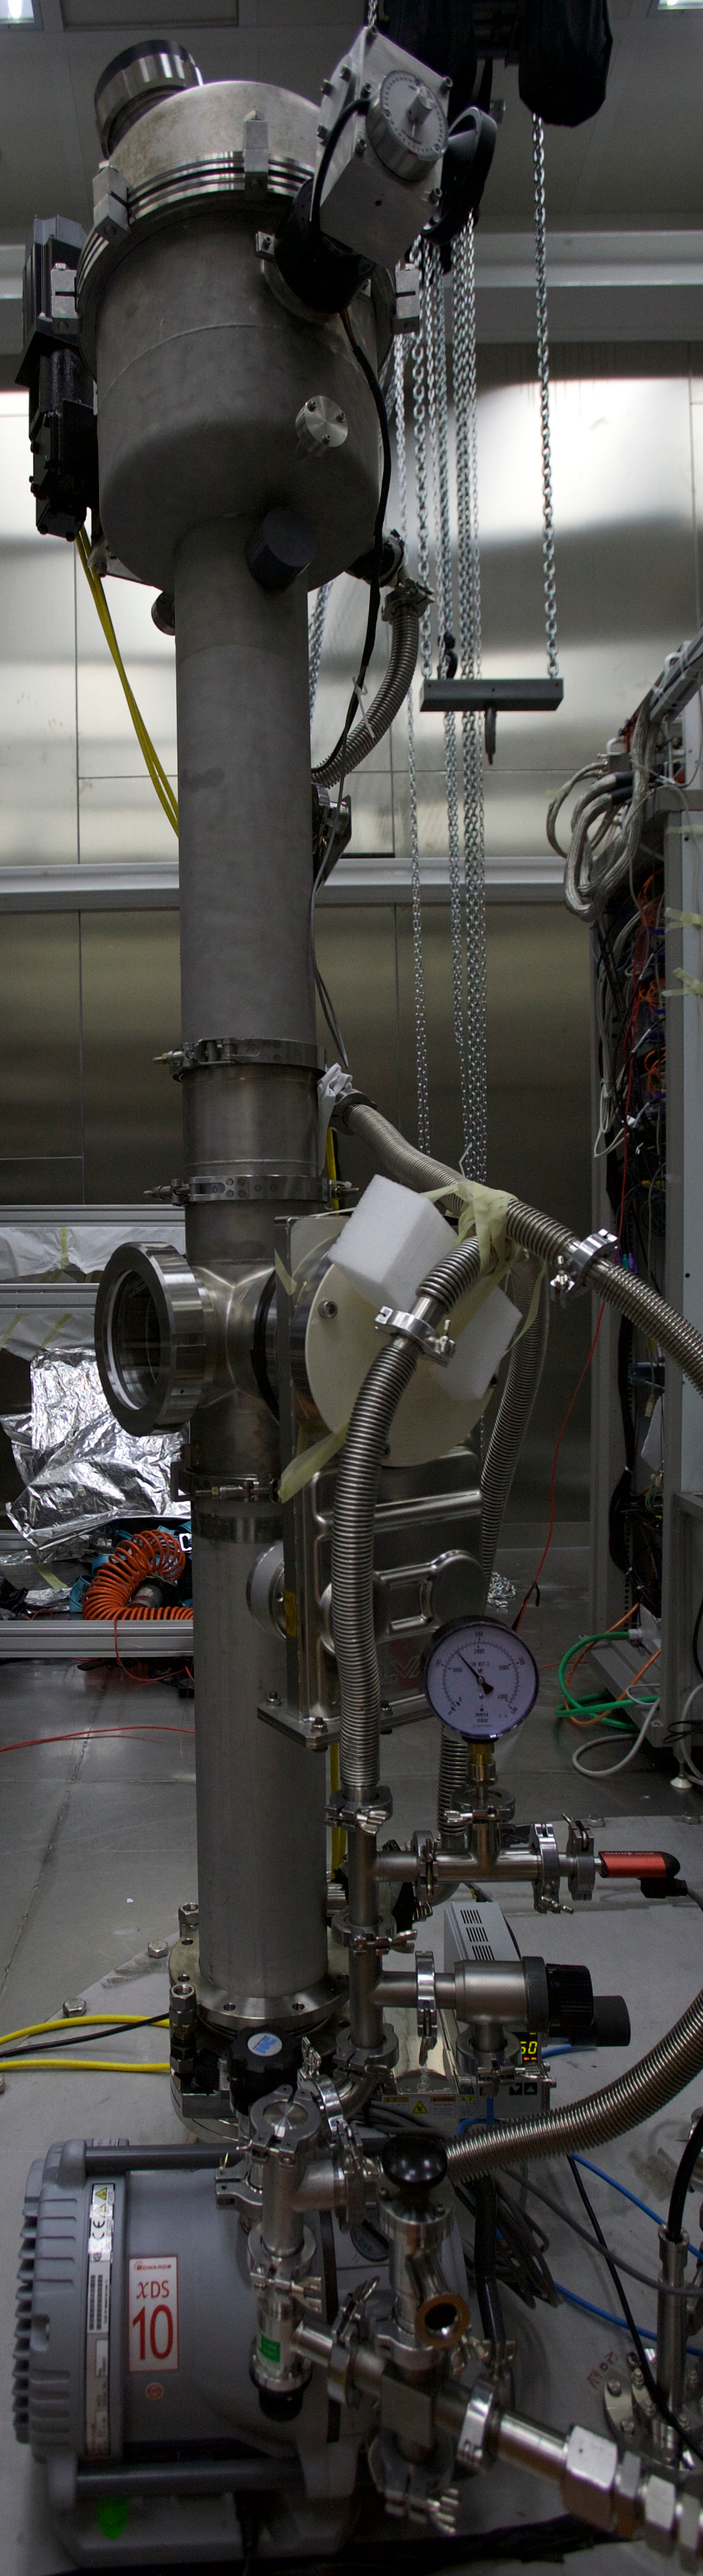
\includegraphics[width=0.30\textwidth]{Figures/CALIS_overview_IMG_3763.jpg}
 \caption{Mechanical drawing of CALIS showing the housing and the deployment device in its home position. The total height is approx.~240 cm including the gate valve.) The two modes of operation are illustrated: In order to move the deployment device down into the LSV or back up the stepper motor moves both cable spools (2) simultaneously. \textcolor{blue}{In order to articulate, the articulation wheel (3) is rotated manually, which affects only the right spool, thereby shortening the right cable with respect to the left cable thereby articulating the arm and lifting the pivot center.} The amount of lifting and the amount of rotations until a horizontal articulation is reached has been calibrated prior to installation in CRH (Sec.~\ref{sec:Testing}). In the photograph the vacuum pump (6) and tubing (7) are shown, which are part of the evacuation and purging system (Sec.~\ref{sec:EvacPurge}). \label{fig:CALISDimensions}\label{fig:CALISMechanism}\label{fig:gearDrawing}\label{fig:flushing_purging}
}
\end{figure}

\begin{figure}[htbp]
 \centering
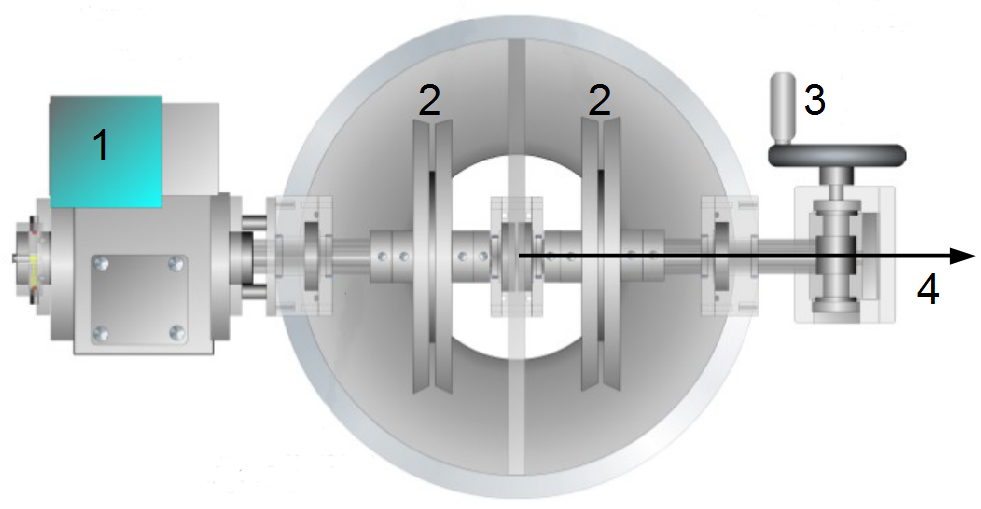
\includegraphics[width=0.9\textwidth]{Figures/gearDrawing_withNumbers}
  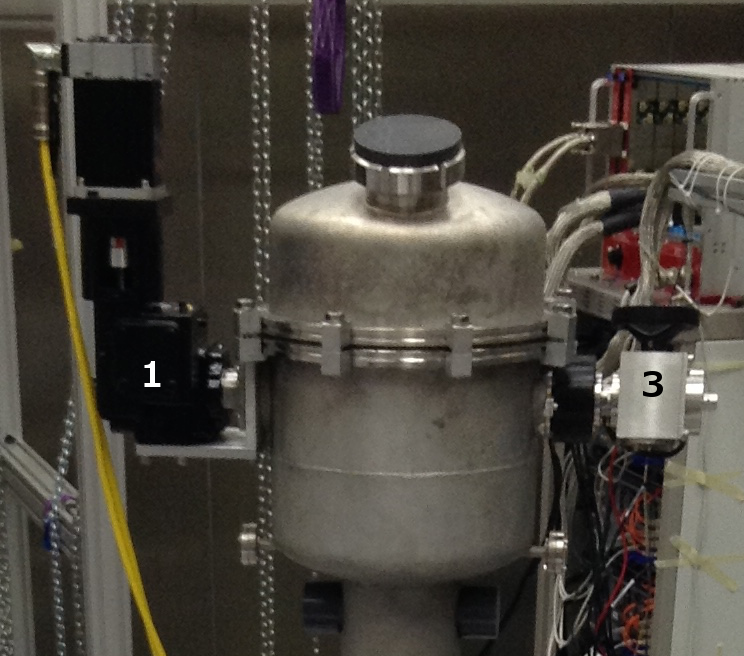
\includegraphics[width=0.46\textwidth]{Figures/CALIS_head.png}
  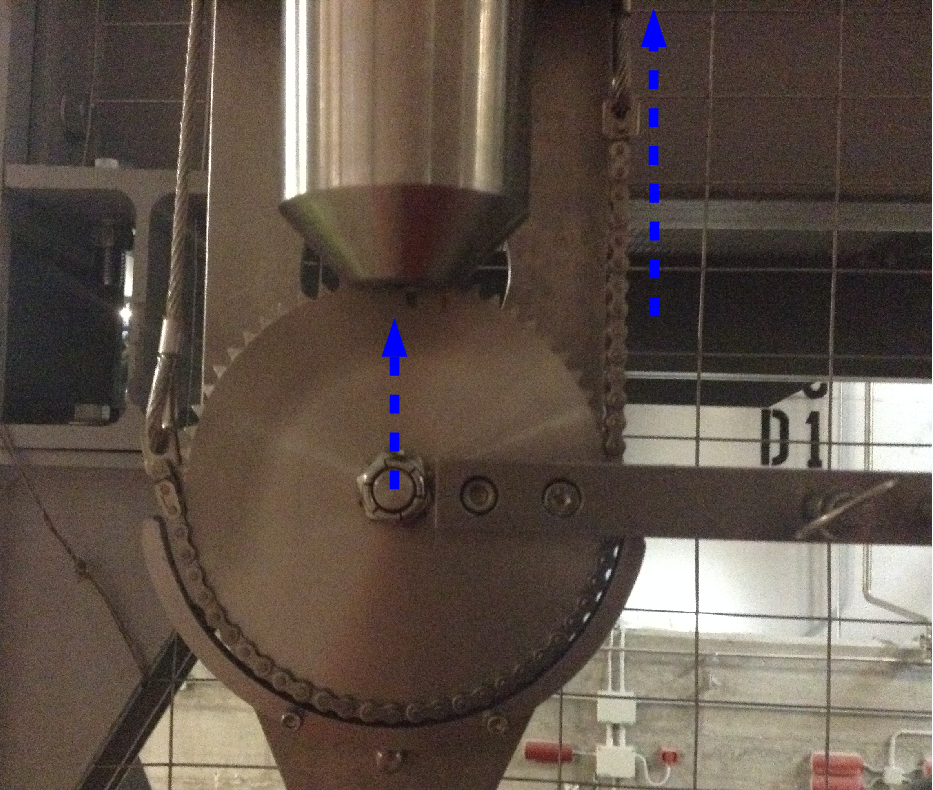
\includegraphics[width=0.48\textwidth]{Figures/gearArticulated.png}
  \caption{\textit{top}: Inside view of drive mechanism's components seen from top of CALIS. Stepper motor inside motor housing (1) drives both cable spools (2) concurrently, thereby lowering calibration device into \lsv. An absolute encoder provides deployment device's current position. Hand wheel (3) turns right spool only, thereby transfering the rotation of articulation wheel into a (de)articulation of the source arm (\textit{bottom right}). Arrow (4) in the sketch points in same direction as horizontally articulated arm. Chain has a guard rail, ensuring chain can never come off the gear.}
  \label{fig:sourceArmRotation}
\end{figure} 

A stepper motor moves both cable spools concurrently and sends deployment device into \lsv. An absolute encoder provides its current position, even in absence of power. The stepper motor is controlled via a simple graphical LabVIEW interface, run on a dedicated laptop, in which current Z-position is shown and a target Z-position can be provided by the operator. Z-positions are given in motor step counts, an arbitrary unit which has been calibrated outside CRH in meters (Fig.~\ref{fig:z_test}) and relative to TPC using calibration data's t-drift distributions (Fig.~\ref{fig:SourcePosition}).

\begin{figure}[htbp]
 \centering
 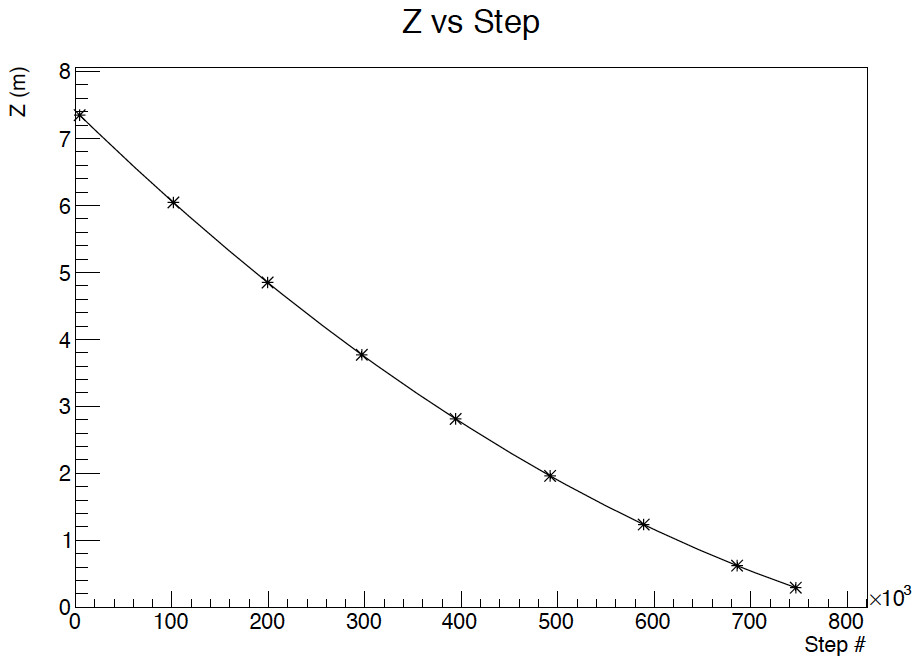
\includegraphics[width=0.65\textwidth]{Figures/Z_positioning_test}
 \caption{Plot of deployment device's Z-position versus motor's step position. Non-linear correspondence between number of steps and cable length deployed arises as follows: As cable winds around spool, the winding radius changes, increasing as deployment device is lifted and decreasing as it is lowered. A motor step count corresponds to a fixed angular distance \textit{d$\theta$}, yet amount of cable deployed during this motor step count is \textit{winding radius $\cdot$ d$\theta$}. As winding radius changes as a function of Z-position, fraction of deployed cable per motor step count changes.}
 \label{fig:z_test}
\end{figure}

\label{sec:Nonlinearity:MotorStepCounts}
Arm articulation is done manually via articulation wheel. This affects only cable spool close to articulation wheel, the left one in Fig.~\ref{fig:sourceArmRotation}, thereby shortening right cable with respect to the left cable and engaging gear through a chain (Fig.~\ref{fig:sourceArmRotation}). As a result arm is articulated and pivot center is lifted. Non-linearity arising from the change in winding radius on cable spools affects also amount of rotation required by hand wheel for horizontal source arm articulation.
Degrees on the articulation wheel corresponding to a horizontal articulation have been calibrated as a function of cable length deployed prior to installation in CRH.

Articulation and a movement in z-direction are mutually exclusive since arm articulation leads to more wound up cable on spool close to articulation wheel with respect to the other. If then in deployment mode both spools would be rotated simultaneously with same angular speed, cable close to articulation wheel would wind up faster than the other, leading to a build up of difference in cable length and the deployment device would only be hanging on one cable. In order to avoid an imbalanced z-movement arm has to be dearticulated fully before a change in z-position can be initiated. This is enforced by an electric switch preventing z-movement, which is disengaged only when arm is fully dearticulated (vertical). 

%Discussion:
% why no permanent tube?
% To complement studies of nuclear recoils with neutron sources ($^{241}$Am$^{9}$Be and $^{241}$Am$^{13}$C), it is planned to deploy a 

\subsection{CALIS Enclosure \& Scintillator}

Besides providing mechanical support for deployment device via cable spools, the CALIS enclosure is an important interface between radon-free clean room CRH and \lsv, through which sources are exchanged. 
The enclosure protects liquid scintillator (LS) and eliminates human contact with any traces of harmful LS vapor (Fig.~\ref{fig:CALISMechanism}). It plays same role as a glove box for similar calibration systems yet with a narrower foot print inside CRH. Liquid scintillator is a mixture of PC and TMB\footnote{The concentration of TMB has varied during campaigns (see Sec.~\ref{sec:CalibCampaigns}).} with the wavelength shifter PPO \cite{Agnes:2015qyz}. %\cite{vetoPaper}. 
It may not get exposed to oxygen or water as is present in normal clean room air. Contamination of LS with $^{222}$Rn and its long-lived radioactive daughters has to be avoided, too. 

Going up from gate valve on which CALIS has been installed, there is a teflon disk that can electrically isolate CALIS from ground, even though during normal operations CALIS housing is connected to ground. A tripod with a bellow has been used to vertically align enclosure right after installation on gate valve. Bellow is connected to a 59.4 cm long cylindrical stainless steel enclosure pipe. It has same diameter as an organ pipe (15 cm) and connects to the view port above by a ring clamp, which plays a critical role in XY-rotations (see Sec.~\ref{sec:XYrotation}). View port can be opened for handling source arm and exchanging sources. Everything above ring clamp forms upper assembly. It features a stainless steel cylindrical enclosure housing cable drive mechanism, including cable spools, stepper motor and articulation mechanism already described in Sec.~\ref{sec:DeploymentArticulation}. 

\subsubsection*{Vacuum evacuation (flushing) and nitrogen purging system}\label{sec:EvacPurge}
One of this system's most important safety features is making sure that TMB and PC residue on device are extracted from CALIS prior to opening access ports to exchange source or arms. This is  important for safe working conditions inside CRH as well as for the scintillator and radiopurity. 

After source arm insertion and view port closure inside of CALIS housing is filled with normal air, that is damaging to the scintillator. A sequence of evacuations and nitrogen purges reduces fraction of air including its contaminants (water vapor, oxygen, radioactivity) to negligible levels. Only after this sequence is finalized gate valve is opened and deployment device is introduced into \lsv. Evacuation is achieved with a vacuum pump and exhaust air is removed through dedicated vent lines (Fig.~\ref{fig:flushing_purging}).

At calibration campaign's end, after deployment device has returned to its home position inside enclosure and gate valve has been closed, scintillator vapor, and in particular TMB, has to be removed prior to opening view port. Again an evacuation and nitrogen purges sequence is employed. By lowering pressure inside of CALIS below TMB and PC vapor pressure, scintillator evaporates and gets removed through vacuum pump vent line. Once pressure inside housing stays consistently below vapor pressure of TMB all scintillator has been removed and view port can be opened to access source arm.
 
%\begin{figure}[htbp]
%\centering
% 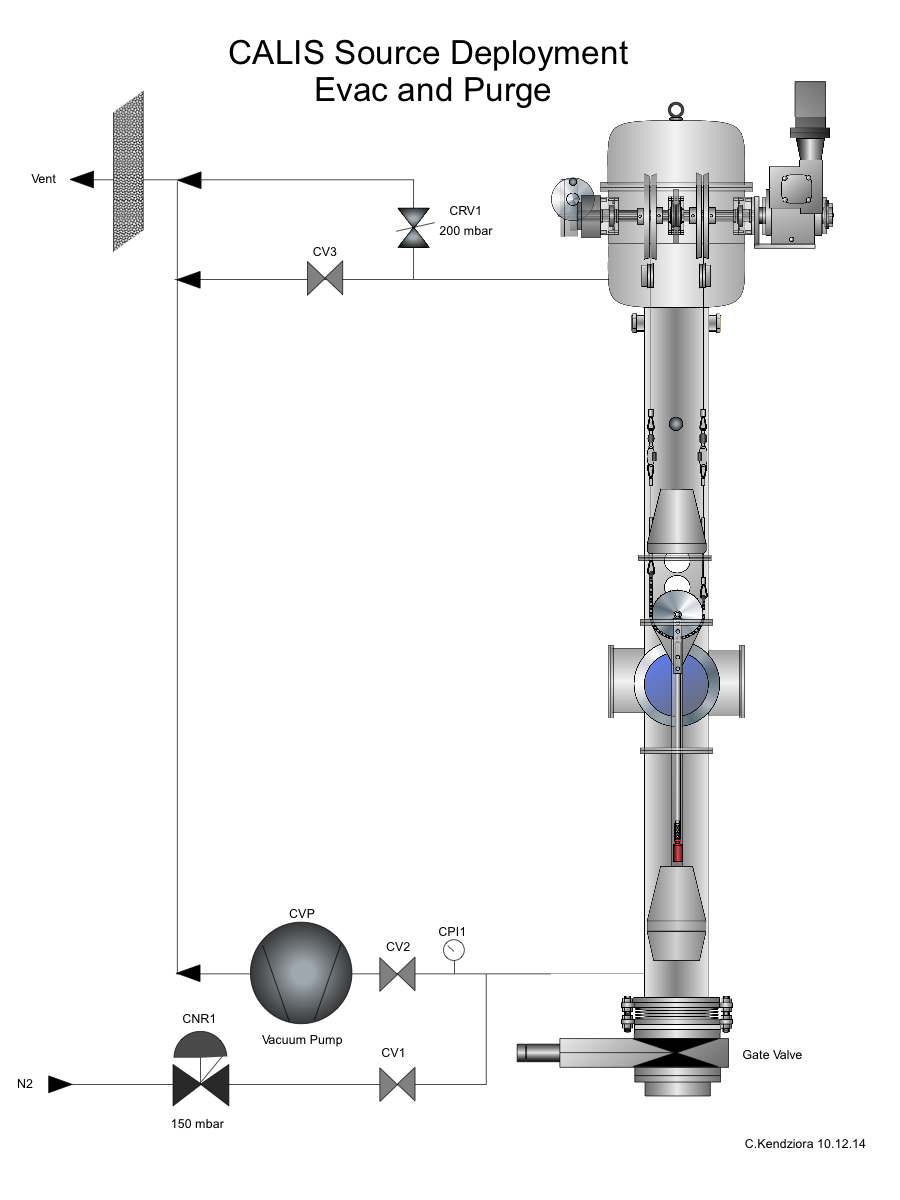
\includegraphics[width=0.73\textwidth]{Figures/GasSystem.png}
% 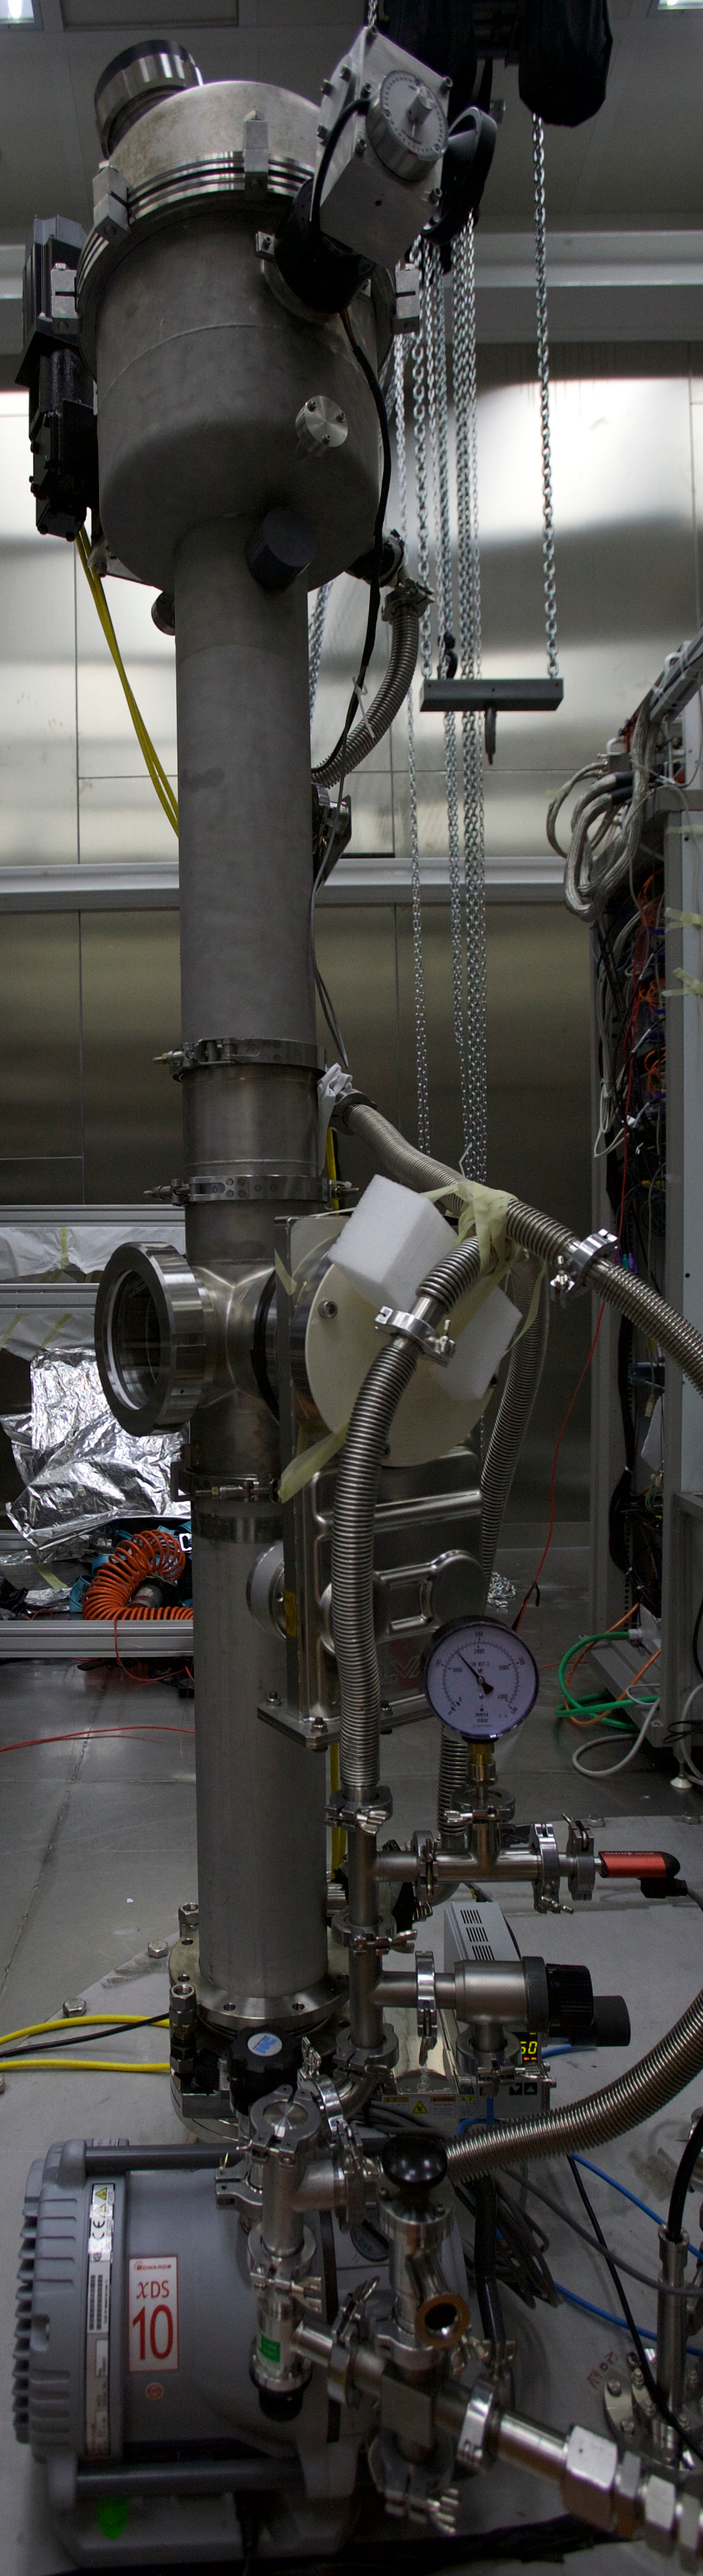
\includegraphics[width=0.25\textwidth]{Figures/CALIS_overview_IMG_3763.JPG}
% \caption{Flushing and nitrogen purging system.}
% \label{fig:flushing_purging}
%\end{figure}

\subsubsection*{Material Compatibility}
All materials coming in contact with scintillator veto are made of stainless steel and teflon except for sealing o-rings which are made of viton.  All three materials are certified materials for contact with all scintillator components including TMB and PC.

\subsection{Deployment Device}
Deployment device (Fig. \ref{fig:CALISMechanism}) contains arm support structure which holds source at its end. Device is equipped with tapered cones on its top and bottom ensuring that ends do not get snagged on organ pipe's inner edges as it moves down and up. It is attached to housing by two cables.  Swivel hooks are employed in cables' attachment to deployment device allowing cables to move freely and not get tangled. 
There are two weights built into the device, one cylindrical in conical cap above rotation gear mechanism and one inside cones at device's bottom end. Both help to minimize any lateral motion or oscillations during deployment, articulation and dearticulation especially. It also ensures smooth motion of deployment device into organ pipe and back to home position inside CALIS housing.

\subsection{Source Holder and Arms}
A source arm and source holder are attached to an articulation gear (Fig.~\ref{fig:SourceHolder}). Different arm lengths have been prepared with a maximum 62 cm arm length, arm length thereby being measured from pivot point of rotation gear to source holder's tip. This arm length allows source to be placed in immediate contact with cryostat (Fig.~\ref{fig:CALIS_photos}, right), as organ pipe's center axis is 80 cm from TPC center and cryostat has an outer radius of 32 cm. The 62 cm arm was used for deployments in past calibration campaigns (Sec.~\ref{sec:CalibCampaigns}). Inside source holder radioactive source is placed, pressed to tip and held in place via a spring during deployment, articulation and dearticulation. Source holder is sealed such that no liquid scintillator can enter during deployment. This has also been verified during each source extraction and no liquid traces have been found on its inside.

\begin{figure}[htbp]
 \centering
  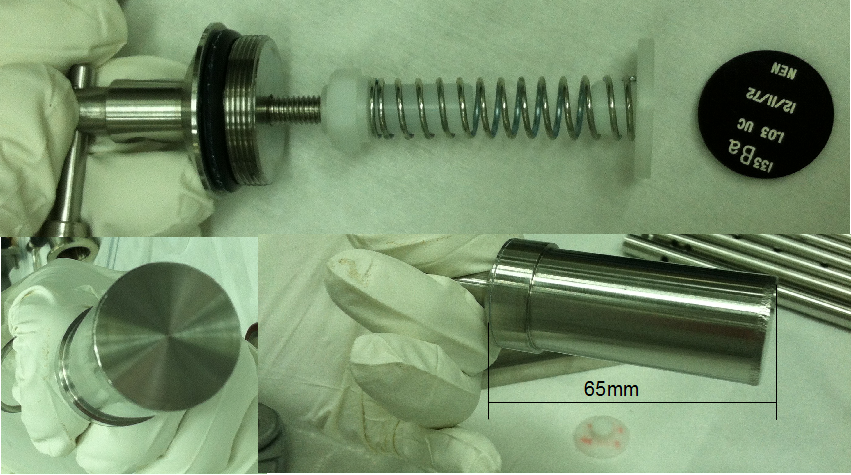
\includegraphics[width=0.7\textwidth]{Figures/SourceHolder.png}
  \caption{Source holder that connects to an arm and to the articulation gear of the deployment device. The source, here a $^{133}$Ba source, is pressed to the tip of the source holder via a spring.}
  \label{fig:SourceHolder}
\end{figure}